\chapter*{Appendix}
\addcontentsline{toc}{chapter}{Appendix}

\section{Results for Cross-Validation}


\begin{figure}[hb!]
\centering
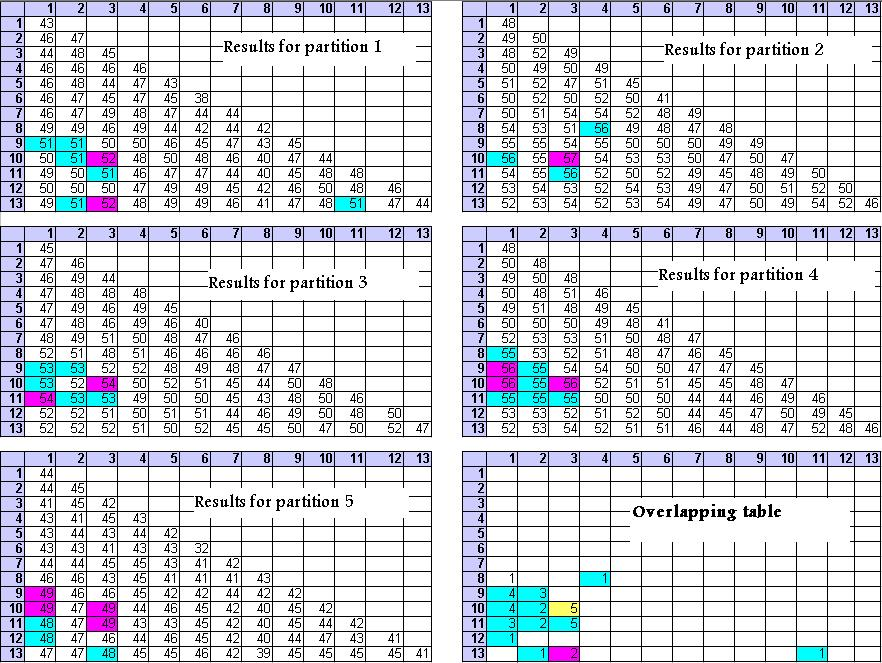
\includegraphics[scale = 0.85]{IB4010_optimisation.jpg}
\caption{Using 5-fold Cross-Validation for parameter optimisation for IB4010}
\label{Using 5-fold Cross-Validation for parameter optimisation for IB4010}
\end{figure}

\pagebreak


\begin{figure}[hb!]
\centering
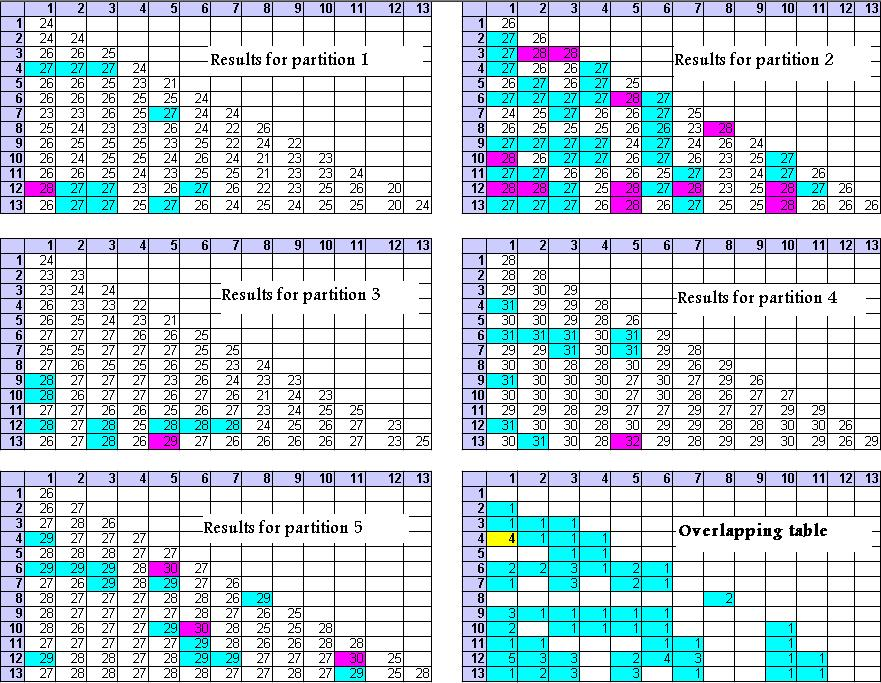
\includegraphics[scale = 0.85]{IS1008c_optimisation.jpg}
\caption{Using 5-fold Cross-Validation for parameter optimisation for IS1008c}
\label{Using 5-fold Cross-Validation for parameter optimisation for IS1008c}
\end{figure}

The two figures above show the results in detail for the section Parameter Optimization over the two meetings, IB4010 and IS1008c. Following the Cross-Validation method, the set of questions is divided into 5 partitions and the results for each partition are described in the figures. There are 6 tables for each meeting in which 5 tables contain the results for 5 partitions respectively and the last table contains the collected results from 5 partitions. The row and the column of each table are the step and the size of search window respectively. In the 5 tables for the results of partitions, the value of each cell is the average number of correct passages for the subset of questions with the parameters corresponding to the row and the column. Meanwhile, in the last table, the value of each cell is the number of the highest values from 5 partitions overlapped for the same parameters.

%What goes in the appendices? Any material which impedes the smooth development of your
%presentation, but which is important to justify the results of a thesis. Generally it is material
%that is of too nitty-gritty a level of detail for inclusion in the main body of the thesis, but which
%should be available for perusal by the examiners to convince them sufficiently. Examples include
%program listings, immense tables of data, lengthy mathematical proofs or derivations, etc.

%\section{Source code in Java}
%\subsection{Calculating passage score}
%
%\lstset{numbers=left, stepnumber=1,breaklines=true}%,basicstyle=\footnotesize ,numberstyle=\footnotesize , showspaces=false, showstringspaces=false, showtabs=false, breakatwhitespace=true }
%
%\lstset{language=Java, caption=Calculating Passage Score, label=DescriptiveLabel}
%\lstset{frame=shadowbox, rulesepcolor=\color{blue}}
%%\begin{frame}
%\lstinputlisting{code.java}
%%\end{frame}
%
%
%\section{Source code of the procedure Determining True Statement}
%%\begin{framed}
%%\begin{lstlisting}…\end{lstlisting}
%%or \lstinputlisting{…}
%%\end{framed}


\section{List of stopwords}
The stopwords that were removed from the transcripts and the questions are listed as below: 

\small 
\textit{i, a, about, above, an, are, as, at, am, and, be, been, being, but, by, do, does, done, did, for, he, her, hers, herself, his, him, himself, how, in, is, it, its, itself, me, my, mine, myself, nor, of, on, or, our, ours, ourself, ourselves, so, she, that, the, they, them, their, theirs, these, themself, themselves, this, those, to, uh, um, up, us, really, very, was, were, we, well, will, with, what, when, where, which, who, whom, whose, why, yet, you, your, yours, yourself, yourselves.
}
\normalsize

\pagebreak

\section{Part-of-speech tags}

\begin{table}[htbp]
\scriptsize
\caption{POS tags used by the QTAG tagger}
\begin{tabular} {|lp{4cm}|lp{4cm}|lp{8cm}|lp{0cm}|} %{|l|l|l|l|}
\hline
\textbf{POS } & \textbf{description } & \textbf{POS } & \textbf{description } \\ \hline
BE & be & PN & pronoun, indefinite \\ \hline
BEDR & were & POS  & possessive particle \\ \hline
BEDZ & was & PP & pronoun, personal \\ \hline
BEG & being & PP\$ & pronoun, possessive \\ \hline
BEM & am & PPX & pronoun, reflexive \\ \hline
BEN & been & RB & adverb, general \\ \hline
BER & are & RBR & adverb, comparative \\ \hline
BEZ & is & RBS & adverb, superlative \\ \hline
CC & conjunction, coordinating & PP & adverbial particle \\ \hline
CD & number, cardinal & SYM & symbol or formula \\ \hline
CS & conjunction, subordinating & TO & infinitive marker \\ \hline
DO & do & UH & interjection \\ \hline
DOD & did & VB & verb, base \\ \hline
DOG & doing & VBD & verb, past tense \\ \hline
DON & done & VBG & verb, -ing \\ \hline
DOZ & does & VBN & verb, past participle \\ \hline
DT & determiner, general & WBZ & verb, -s \\ \hline
EX & existential there & WDT & det, wh- \\ \hline
FW & foreign word & WP & pronoun, \\ \hline
HV & have & WP\$ & pronoun, possessive \\ \hline
HVD & had & WRB & adv, wh- \\ \hline
HVG & having & XNOT & negative marker \\ \hline
HVN & had & ! & exclamation mark \\ \hline
HVZ & has & ' & quotation mark \\ \hline
IN & preposition & ' & apostrophe \\ \hline
JJ & adjective, general & ( & parenthesis begin \\ \hline
JJR & adjective, comparative & ) & parenthesis end \\ \hline
JJS & adjective, superlative & , & comma \\ \hline
MD & modal auxiliary & - & dash \\ \hline
NN & noun, common singular & . & point \\ \hline
NNS & noun, common plural & ... & ... \\ \hline
NP & noun, proper singular & : & colon \\ \hline
NPS & noun, proper plural & ; & semi-colon \\ \hline
OD & number, ordinal & ? & question mark \\ \hline
PDT & determiner, pre- & ??? & undefined \\ \hline
\end{tabular}
\label{PoS}
\end{table}
